\section{Experimental procedures}
We perform several experiments using the model "stable-diffusion-v1-5" by runwayml\cite{Rombach_2022_CVPR} and applying different kinds of token merging to a set of prompts and measuring the performance.
The performance is defined by\\ 
\(1)\) speed: the average diffusion time for every image of the set and\\
\(2)\) image quality: the FID-value between sets of images that had token merging applied and their counterparts (that is same prompt, seed and image size) that didn't use any token merging.

\subsection{Setup}
\subsubsection*{Software}
The first iteration of the experiment was to compare how diffusion time and image quality change across a spectrum of different volume of tokens  removed while token merging is applied in different layers of the transformer (self-attention, cross-attention and mlp).\\
The images were generated with a "DiffusionPipeline" from HuggingFace's diffusers library using the "stable-diffusion-v1-5" model\cite{Rombach_2022_CVPR}.\\
We sampled a set of \(n=500\) prompts from the dataset "Gustavosta/Stable-Diffusion-Prompts" on HuggingFace which has 80,000 prompts filtered and extracted from the image finder for Stable Diffusion: "Lexica.art".\\
Seven 768x768 images were created per prompt with a 0\%, 10\%, 20\%, 30\%, 40\%, 50\% and 60\% merge applied respectively, creating a set of 3,500 images which can be split up into 7 subsets of 500 images each for every merge volume.\\
This experiment was run multiple times with the merges applied in different layers of the transformer to compare performance.

\subsubsection*{Hardware}
All experminents were conducted on Nvidida GeForce GTX 1080 Ti GPUs. Individual images were always created on single GPUs.

\subsection{Adjustments}
\subsubsection*{FID}
We created and used our own fork of pytorch-fid\cite{Seitzer2020FID} to accommodate for the hpc not being connected to the internet and therefore not being able to download the weights of the Inception model to calculate FID-values. Our fork loads these weights from a local directory to avoid any connection to the internet and requires the user to have them pre-installed.

\subsubsection*{Prompts}
We shortened every prompt thats exceeds 300 characters in order to reduce the number of tokens to a maximum of 77, as CLIP\cite{radford2021learning} can only handle up to 77 tokens.\\
This is done by determining the index (\(idx\)) of the last comma in the first 300 characters of every prompt and then cutting off everything from this point onwards.
\begin{lstlisting}[language=Python]
prompt = prompt[:idx]
\end{lstlisting}

\subsection{Comparison to original setup}
Text.

\subsection{Results}

% FID values for run2 and run3
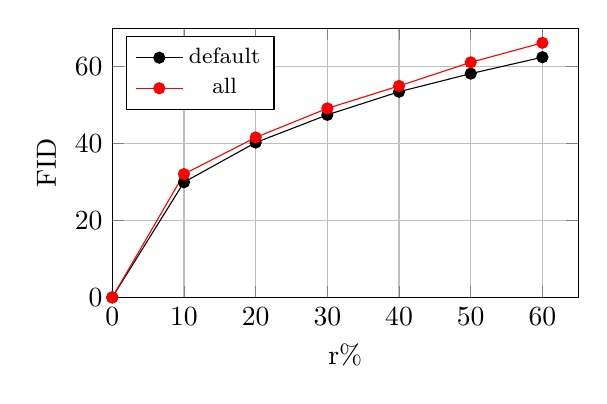
\begin{tikzpicture}
\begin{axis}[
    title={},
    height=5cm,
    width=7.5cm,
    xlabel={r\%},
    ylabel={FID},
    xmin=0, xmax=65,
    ymin=0, ymax=70,
    xtick={0,10,20,30,40,50,60},
    ytick={0,20,40,60},
    legend pos=north west,
    xmajorgrids=true,
    ymajorgrids=true,
    legend style={font=\footnotesize}
]

\addplot[
    color=black,
    mark=*
    ]
    coordinates {
    (0,0)(10,29.95)(20,40.26)(30,47.47)(40,53.48)(50,58.19)(60,62.46)
    };
    
\addplot[
    color=red,
    mark=*
    ]
    coordinates {
    (0,0)(10,32.07)(20,41.60)(30,49.15)(40,54.99)(50,61.13)(60,66.20)
    };
    
\legend{default, all}
    
\end{axis}
\end{tikzpicture}

\begin{table}
    \centering
    \begin{tabular}{|c|c|c|}
        \hline
        m\_vol (\%) & FID (default) & FID (all) \\
        \hline
        0 & 0 & 0 \\
        10 & 29.95 & 32.07 \\
        20 & 40.26 & 41.60 \\
        30 & 47.74 & 49.15 \\
        40 & 53.48 & 54.98 \\
        50 & 58.19 & 61.13 \\
        60 & 62.46 & 66.21 \\
        \hline
    \end{tabular}
    \caption{Your caption here}
    \label{tab:yourlabel}
\end{table}

% time values for run2 and run3
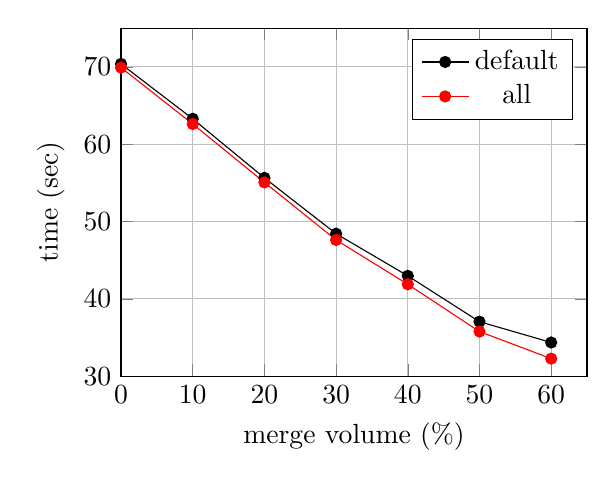
\begin{tikzpicture}
\begin{axis}[
    title={},
    height=6cm,
    width=7.5cm,
    xlabel={merge volume (\%)},
    ylabel={time (sec)},
    xmin=0, xmax=65,
    ymin=30, ymax=75,
    xtick={0,10,20,30,40,50,60},
    ytick={30,40,50,60,70},
    legend pos=north east,
    xmajorgrids=true,
    ymajorgrids=true,
]

\addplot[
    color=black,
    mark=*
    ]
    coordinates {
    (0,70.38)(10,63.28)(20,55.64)(30,48.42)(40,42.97)(50,37.04)(60,34.35)
    };
    
\addplot[
    color=red,
    mark=*
    ]
    coordinates {
    (0,69.91)(10,62.61)(20,55.06)(30,47.61)(40,41.88)(50,35.76)(60,32.26)
    };
    
\legend{default, all}
    
\end{axis}
\end{tikzpicture}

% FID values for run2, run4 and run5
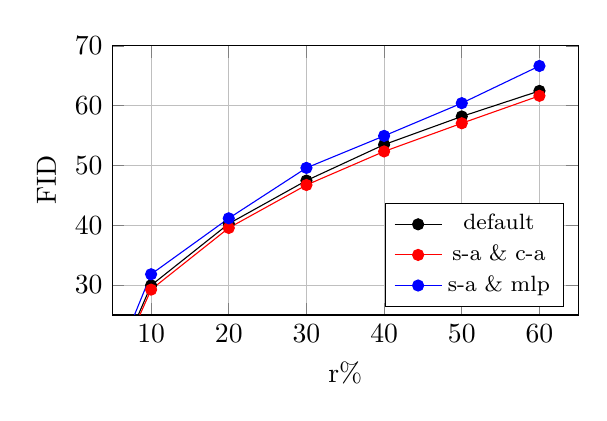
\begin{tikzpicture}
\begin{axis}[
    title={},
    height=5cm,
    width=7.5cm,
    xlabel={r\%},
    ylabel={FID},
    xmin=5, xmax=65,
    ymin=25, ymax=70,
    xtick={10,20,30,40,50,60},
    ytick={30,40,50,60,70},
    legend pos=south east,
    xmajorgrids=true,
    ymajorgrids=true,
    legend style={font=\footnotesize}
]

\addplot[
    color=black,
    mark=*
    ]
    coordinates {
    (0,0)(10,29.95)(20,40.26)(30,47.47)(40,53.48)(50,58.19)(60,62.46)
    };
    
\addplot[
    color=red,
    mark=*
    ]
    coordinates {
    (0,0)(10,29.24)(20,39.55)(30,46.73)(40,52.34)(50,57.05)(60,61.64)
    };

\addplot[
    color=blue,
    mark=*
    ]
    coordinates {
    (0,0)(10,31.81)(20,41.16)(30,49.59)(40,54.94)(50,60.41)(60,66.63)
    };
    
\legend{default, s-a \& c-a, s-a \& mlp}
    
\end{axis}
\end{tikzpicture}

% time values for run2, run4 and run5
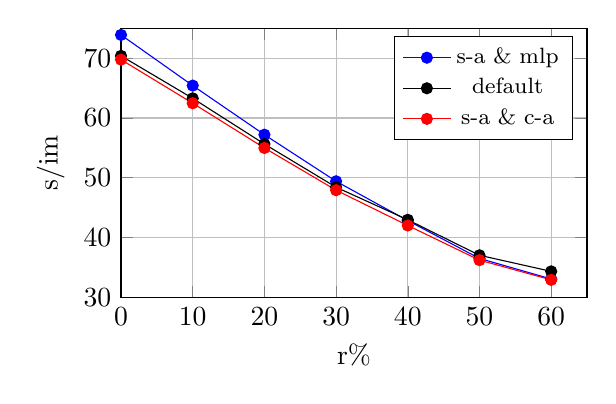
\begin{tikzpicture}
\begin{axis}[
    title={},
    height=5cm,
    width=7.5cm,
    xlabel={r\%},
    ylabel={s/im},
    xmin=0, xmax=65,
    ymin=30, ymax=75,
    xtick={0,10,20,30,40,50,60},
    ytick={30,40,50,60,70},
    legend pos=north east,
    xmajorgrids=true,
    ymajorgrids=true,
    legend style={font=\footnotesize}
]

\addplot[
    color=blue,
    mark=*
    ]
    coordinates {
    (0,73.88)(10,65.41)(20,57.20)(30,49.41)(40,42.83)(50,36.51)(60,33.08)
    };

\addplot[
    color=black,
    mark=*
    ]
    coordinates {
    (0,70.38)(10,63.28)(20,55.64)(30,48.42)(40,42.97)(50,37.04)(60,34.35)
    };
    
\addplot[
    color=red,
    mark=*
    ]
    coordinates {
    (0,69.75)(10,62.46)(20,54.98)(30,47.92)(40,42.02)(50,36.23)(60,32.93)
    };

    
\legend{s-a \& mlp, default, s-a \& c-a}
    
\end{axis}
\end{tikzpicture}

\subsection{Comparison to original results}
Text.